\documentclass[conference]{IEEEtran}
\usepackage[top=3cm, bottom=2cm, left=2cm, right=2cm, columnsep=20pt]{geometry}
\usepackage{pdfpages}
\usepackage{graphicx}
\usepackage{etoolbox}
\apptocmd{\sloppy}{\hbadness 10000\relax}{}{}
% \usepackage[numbers]{natbib}
\usepackage[T1]{fontenc}
\usepackage{ragged2e}
\usepackage[french]{babel}
\usepackage{listings}
\usepackage{color}
\usepackage{soul}
\usepackage[utf8]{inputenc}
\usepackage[export]{adjustbox}
\usepackage{caption}
\usepackage{mathrsfs, amsmath}
\usepackage{amssymb}
\usepackage{float}
\usepackage{csquotes}
\usepackage{fancyhdr}
\usepackage{wallpaper}
\usepackage{siunitx}
\usepackage[indent]{parskip}
\usepackage{textcomp}
\usepackage{gensymb}
\usepackage{multirow}
\usepackage[hidelinks]{hyperref}
\usepackage{abstract}
\usepackage{subcaption}
\usepackage{tabularx}
\usepackage{biblatex}
\addbibresource{bibliographie.bib}

% \renewcommand{\abstractnamefont}{\normalfont\bfseries}
% \renewcommand{\abstracttextfont}{\normalfont\itshape}
\usepackage{titlesec}
% \titleformat{\section}{\large\bfseries}{\thesection}{1em}{}
% \titleformat{\subsection}{\normalsize\bfseries}{\thesubsection}{1em}{}
% \titleformat{\subsubsection}{\normalsize\bfseries}{\thesubsubsection}{1em}{}

\usepackage{xcolor}
\definecolor{codegreen}{rgb}{0,0.6,0}
\definecolor{codegray}{rgb}{0.5,0.5,0.5}
\definecolor{codepurple}{rgb}{0.58,0,0.82}
\definecolor{backcolour}{rgb}{0.95,0.95,0.92}
\lstdefinestyle{mystyle}{
    backgroundcolor=\color{backcolour},   
    commentstyle=\color{codegreen},
    keywordstyle=\color{magenta},
    numberstyle=\tiny\color{codegray},
    stringstyle=\color{codepurple},
    basicstyle=\ttfamily\footnotesize,
    breakatwhitespace=false,         
    breaklines=true,                 
    captionpos=b,                    
    keepspaces=true,                 
    numbers=left,                    
    numbersep=5pt,                  
    showspaces=false,                
    showstringspaces=false,
    showtabs=false,                  
    tabsize=2
}
\lstset{style=mystyle}

\usepackage[most]{tcolorbox}
\newtcolorbox{note}[1][]{
  enhanced jigsaw,
  borderline west={2pt}{0pt}{black},
  sharp corners,
  boxrule=0pt, 
  fonttitle={\large\bfseries},
  coltitle={black},
  title={Note:\ },
  attach title to upper,
  #1
}


%----------------------------------------------------

\setlength{\parindent}{0pt}
\DeclareCaptionLabelFormat{mycaptionlabel}{#1 #2}
\captionsetup[figure]{labelsep=colon}
\captionsetup{labelformat=mycaptionlabel}
\captionsetup[figure]{name={Figure }}
\captionsetup[table]{name=Tableau}
\newcolumntype{Y}[1]{>{\Centering\hspace{0pt}\hsize=#1\hsize}X}
\newcommand{\inlinecode}{\normalfont\texttt}
\usepackage{enumitem}
\setlist[itemize]{label=\textbullet}

\begin{document}

%----------------------------------------------------
\title{Spectromètre\\
\large Travail préparatoire \\
PHS3910 -- Techniques expérimentales et instrumentation\\ 
Équipe L3}

\author{\IEEEauthorblockN{Émile Guertin-Picard}
\IEEEauthorblockA{2208363}
\and
\IEEEauthorblockN{Maxime Rouillon}
\IEEEauthorblockA{2213291}
\and
\IEEEauthorblockN{Marie-Lou Dessureault}
\IEEEauthorblockA{2211129}
\and
\IEEEauthorblockN{Philippine Beaubois}
\IEEEauthorblockA{2211153}
}

\maketitle

\textit{\textbf{Résumé} -- yap yap}

\section{Introduction}
yap yap

\section{Méthodes \label{methodes}}

Le système optique du spectromètre est schématisé dans la figure \ref{4f}.

\begin{figure}[H]
    \centering
    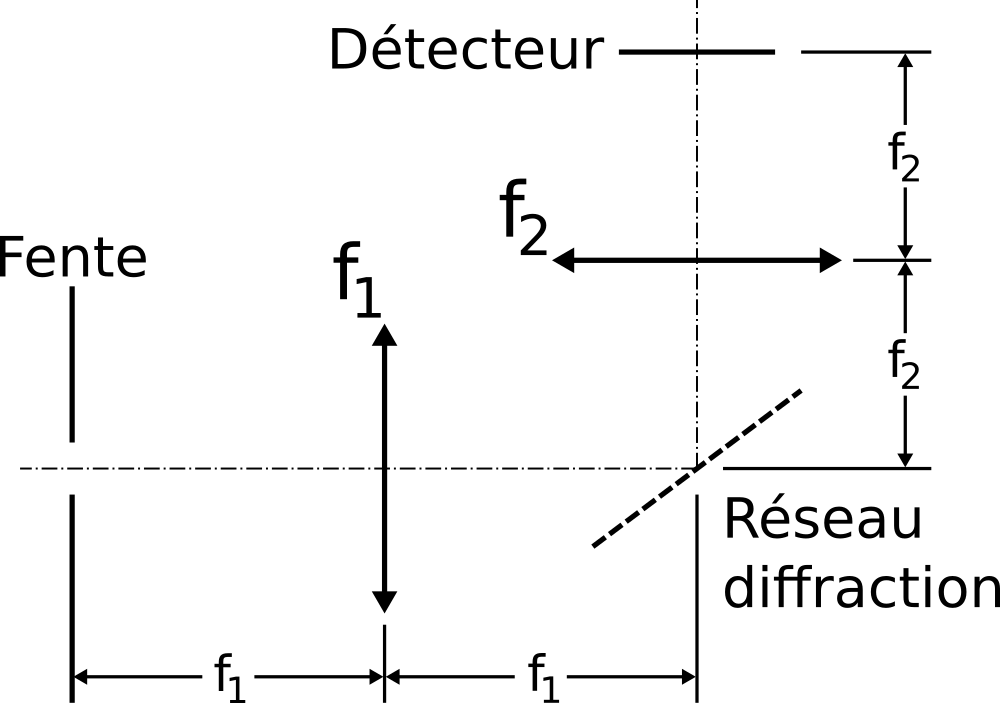
\includegraphics[scale=0.4]{4f.png}
    \caption{Schéma simplifié du spectromètre avec toutes ses composantes \cite{procedurier}. \label{4f}}
\end{figure}

Le parcours d'un faisceau passant à travers le spectromètre a été simulé à l'aide 
de l'optique de Fourier. Le champ initial a été modélisé par une fonction rectangle en deux dimensions,
afin de modéliser la forme du champ après avoir traversé une fente. Celui-ci peut donc être décrit par:
\[U(x_0,y_0)=rect(\frac{y_0}{b})rect(\frac{x_0}{a}),\]
où $a$ et $b$ sont la largeur et la hauteur de la fente respectivement. Le champ transmis par 
la première lentille a donc pu être déterminé:

\begin{align*}
    U_1(x_1,y_1)&\propto\mathscr{F}\left\{U(x_0,y_0)\right\}(\frac{x_1}{\lambda f_1},\frac{y_1}{\lambda f_1})\\
    &\propto \mathscr{F}\left\{rect(\frac{y_0}{b})rect(\frac{x_0}{a})\right\}(\frac{x_1}{\lambda f_1},\frac{y_1}{\lambda f_1})\\
    &\propto sinc(\frac{y_1b}{\lambda f_1})\ast sinc(\frac{x_1a}{\lambda f_1}),
\end{align*}
où $f_1$ est la longueur focale de la lentille. Le réseau de diffraction blazé modifie la forme du champ, ce qui a pu être
modélisé à l'aide d'un masque \cite{procedurier}:
\[M(x_1,y_1)=(comb(\frac{x_1}{\Lambda})\ast rect(\frac{x_1}{\Lambda})e^{i\beta x})rect(\frac{x_1}{N\Lambda}).\]

Ici, la forme du champ n'est pas limitée par la grandeur du réseau de diffraction, mais par les dimensions
de la fente; le terme $rect(x_1/N\Lambda)$ a pu être négligé. Le champ à la sortie de la deuxième lentille revient à effectuer la transformée de Fourier
de $U_1(x_1,y_1)$:

\begin{align*}
    U_2\propto&\ \mathscr{F}\left\{sinc(\frac{y_1b}{\lambda f_1})\ast sinc(\frac{x_1a}{\lambda f_1})M\right\}(\frac{x_2}{\lambda f_2},\frac{y_2}{\lambda f_2})\\
    \propto&\ rect(\frac{y_2 f_1}{b f_2})rect(\frac{x_2 f_1}{a f_2})\ast comb(\frac{x_2 \Lambda}{\lambda f_2})\\
    &\ sinc(\frac{x_2 \Lambda}{\lambda f_2})\ast \delta(2\pi(x_2-\frac{\beta}{2\pi}))\\
    \propto&\ rect(\frac{y_2 f_1}{b f_2})rect(\frac{x_2 f_1}{a f_2})\ast comb(\frac{x_2 \Lambda}{\lambda f_2})\\
    &\ sinc(\frac{\Lambda}{\lambda f_2}(x_2-\frac{\lambda f_2 \beta}{2\pi})).
\end{align*}
Pour évaluer le terme $rect(\frac{x_2 f_1}{a f_2})\ast comb(\frac{x_2 \Lambda}{\lambda f_2})$, la fonction $comb$ a été remplacée par sa définition:
\begin{align*}
    rect(\frac{x_2 f_1}{a f_2})\ast comb(\frac{x_2 \Lambda}{\lambda f_2})&=rect(\frac{y_2 f_1}{b f_2})\ast\sum_{\infty}\delta(x_2-\frac{n\lambda f_2}{\Lambda})\\
    &=\sum_{\infty}rect(\frac{f_1}{a f_2}(x_2-\frac{n\lambda f_2}{\Lambda})).
\end{align*}
En rassemblant tous les termes, on a obtenu:
\begin{align*}
    U_2(x_2,y_2)\propto&\ rect(\frac{y_2 f_1}{b f_2})\sum_{\infty}rect(\frac{f_1}{a f_2}(x_2-\frac{n\lambda f_2}{\Lambda}))\\
    & \ sinc(\frac{\Lambda}{\lambda f_2}(x_2-\frac{\lambda f_2 \beta}{2\pi})).
\end{align*}

On sait que $\beta x = \phi$, où $\phi$ est le décalage de phase entre deux faisceaux à la sortie du réseau de diffraction.
La différence de parcours $\delta(x)$ est directement reliée au décalage de phase par $\phi=2\pi\delta(x)/\lambda$, où $\delta(x)=2tan\theta x$.
Ce résultat est illustré dans la figure \ref{beta}. 

\begin{figure}[H]
    \centering
    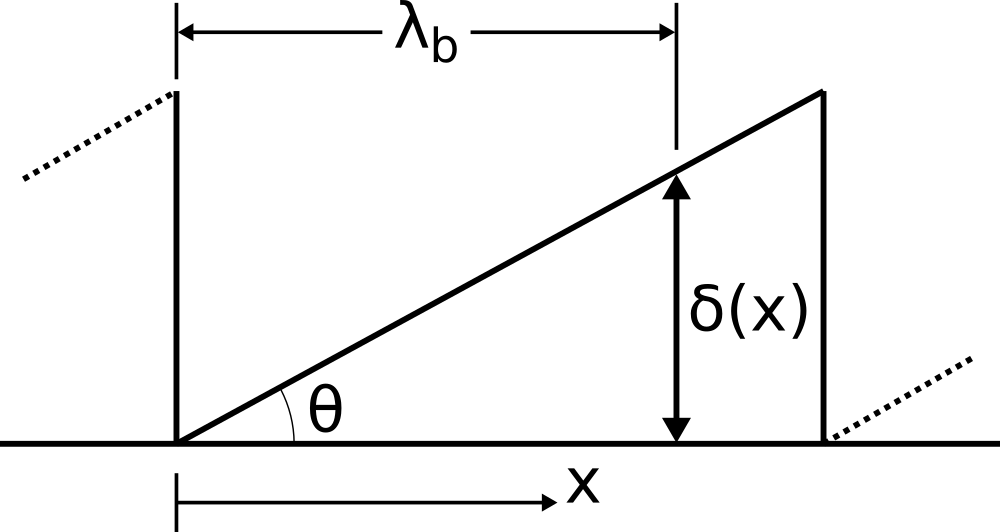
\includegraphics[scale=0.2]{beta.png}
    \caption{Représentation de la différence de parcours de deux faisceaux sur un réseau de diffraction
    blazé. Ici, $\lambda_B$ correspond à la longueur d'onde de Blaze. \label{beta}}
\end{figure}
En faisant l'approximation des petits angles $tan\theta\approx\theta$, on retrouve:
\begin{align*}
   \beta x &=\frac{2\pi\delta(x)}{\lambda} \approx\frac{4\pi\theta x}{\lambda}\\
   \beta&\approx \frac{4\pi\theta}{\lambda}
\end{align*} 

Avec l'équation de Bragg pour la diffraction, et en choisissant l'ordre $m=1$, on a trouvé que $2\Lambda sin\theta=\lambda_B \rightarrow \theta\approx\lambda_B/2\Lambda$.
On a donc:

\begin{align*}
   \beta&\approx \frac{2\pi\lambda_B}{\lambda\Lambda}.
\end{align*}

En remplaçant ce terme dans la fonction $sinc$, on a $sinc(\frac{\Lambda}{\lambda f_2}(x_2-\frac{\lambda_B f_2}{\Lambda}))$. En comparant cette
fonction $sinc$ avec la fonction $rect$ en $x$, on a pu remarquer que le terme $n=1$ de la somme s'aligne parfaitement 
avec la fonction $sinc$ lorsque $\lambda=\lambda_B$, où $\lambda_B$ est la longueur d'onde de Blaze. Par conséquent, on considère que pour des longueurs d'onde proches
de $\lambda_B$, l'ordre $n=1$ est aussi suffisament aligné à la fonction $sinc$. La forme de $sinc$ nous a permis d'éliminer tous les autres termes $n\neq1$, et on a obtenu:

\begin{align*}
    U_2(x_2,y_2)\propto&\ rect(\frac{y_2 f_1}{b f_2})rect(\frac{f_1}{a f_2}(x_2-\frac{\lambda f_2}{\Lambda}))\\
    & \ sinc(\frac{\Lambda}{\lambda f_2}(x_2-\frac{\lambda f_2}{\Lambda})).
\end{align*}

Les largeurs du $sinc$ et du $rect$ en $x$ sont proportionnelles à $\lambda f_2/\Lambda$ et $af_2/f_1$, respectivement, ce qui nous
a permis de traiter $sinc\approx1$ parce que l'ordre de grandeur (pour les contraintes du projet) de $\lambda/\Lambda$ est de $\approx10^{-1}$ alors que celui de $a/f_1$ est
de $\approx10^{-2}$. La forme finale de $U_2(x_2,y_2)$ est:

\begin{align*}
    U_2(x_2,y_2)\propto&\ rect(\frac{y_2 f_1}{b f_2})rect(\frac{f_1}{a f_2}(x_2-\frac{\lambda f_2}{\Lambda})).
\end{align*}

Une contrainte du projet consiste à ce que la largeur du spectre d'ordre 1 capté par la caméra
soit d'une largeur équivalente ou légèrement inférieure à la largeur de la caméra. Mathématiquement, ceci correspond à
$x(\lambda_{bleu})-x(\lambda_{rouge})\leq D_{cam}$. On a pu approximer que $x(\lambda)$ correspond au terme de décalage
de la fonction $rect$ en $x$. Les dimensions de la caméra utilisée pour le spectromètre sont de 1280 x 1024 pixels, chacun étant un carré de
$5.2\ \mu m$ côté. La zone sensible de la caméra est donc de 6.656 x 5.323 mm \cite{camera}. Par conséquent, il a été nécessaire d'optimiser la relation suivante
en fonction des lentilles disponibles (10, 15, 20, 25, 30, 50 ou 100 mm de longueur focale):

\begin{align*}
    \frac{f_2}{\Lambda}(\lambda_{bleu}-\lambda_{rouge})\leq 6.656\ mm.
\end{align*}

Ayant une valeur de $f_2$ déterminée, la résolution du spectromètre a pu ensuite être optimisée. La résolution a été trouvée en
considérant que deux longueurs d'onde voisines, $\lambda_1$ et $\lambda_2$, se touchent à une valeur de $x$ qui correspond à:

\begin{align*}
    x=\frac{a f_2}{2f_1}+\frac{\lambda_1 f_2}{\Lambda}&=-\frac{a f_2}{2f_1}+\frac{\lambda_2 f_2}{\Lambda}\\
    \frac{af_2}{f_1}&=\frac{f_2}{\Lambda}(\lambda_2-\lambda_1)\\
    \delta_{\lambda}&=\lambda_2-\lambda_1=\frac{\Lambda a}{f_1}
\end{align*}
Afin de modéliser l'équation trouver et de la visualiser, un code python a été créé. Celui-ci recrée, à partir de l'équation
de U2, l'image apparaisant sur la caméra. Plusieurs longueurs d'onde du rouge au bleu ont été testées pour vérifer 
la fiabilité de l'équation avec les paramètres obtenus précédement, soit les deux focales ainsi que les dimensions de la fente. 
Ce processus a également permis de prédire l'emplacement des différentes longueurs d'onde sur la caméra 
et ainsi de vérifier si le spectre complet de la lumière visible était présent. Il permet également d'observer les
impacts des différents paramètres sur la forme et l'aspect des images obtenues. Concrètement, le code python prend 
l'équation de U2 et l'implémente sur une grille de la taille du capteur de la caméra. Cette partie permet d'obtenir 
la position et la forme de l'image. Par la suite, la fonction $wavelength\_to\_rgb$ permet de colorer l'image en fonction
de la longueur d'onde envoyé. Ainsi, il est possible de visualiser l'emplacement, la forme et la couleur de l'image.    

Pour déterminer à quel angle positionner le réseau de diffraction pour 
obtenir un axe optique diffracté à 90$^{\circ}$ et , l'équation \ref{GratingEq} a été utilisée \textcolor{red}{reference}:

\begin{align}\label{GratingEq}
    G m \lambda &= \sin(\theta_i) + \sin(\theta')
\end{align}

Où G est le nombre de miroirs par mm, m est l'ordre de diffraction, $\lambda$ est la longueur d'onde,
$\theta_i \ge 0$ est l'angle incident et $\theta' \le 0$ l'angle diffracté. Avec m=1 et $G=600mm^{-1}$, 
on a obtenu les relations entre l'angle d'incidence et l'angle du rayon diffracté pour les deux longueurs 
d'onde extrêmes. Avec la condition $\theta_i-\theta'=90$ et en minimisant la différence entre les angles 
de sortie, on a obtenu l'angle d'incidence optimal qui détermine le positionnement du réseau de diffraction.
L'angle entre la longueur d'onde centrale et l'onde incidente ainsi que la longueur d'onde diffractée 
exactement sur l'axe optique ont pu être determinées une fois l'angle d'incidence obtenu.



\section{Résultats \label{resultats}}
En considérant $\lambda_{bleu}=380\ nm$ et $\lambda_{rouge}=780\ nm$, les largeurs des spectres obtenues sont présentées
dans le tableau \ref{largeur_spectre}. Le terme $\Delta_D$ correspond à l'écart entre le diamètre de la caméra et le diamètre du spectre.
\begin{table}[H]
    \caption{Résultats des largeurs de spectres pour des lentilles ayant des longueurs focales
    $f_2$ de 10, 15, 20, 25, 30, 50 ou 100 mm. Le réseau de diffraction a 600 lignes/mm, ce qui correspond à un pas de réseau
    de $\Lambda=1/600$ mm \cite{grating}.}    
    \centering
    \begin{tabular}{c|c|c|c}
    $\Lambda$ (mm) & $f_2$ (mm) & $D_{spectre}$ (mm) & $\Delta_D$ \\
    \hline
    \hline
    \multirow{7}{*}{1/600} & 10 & 2.40 & -4.256 \\
    & 15 & 3.60 & -3.056 \\
    & 20 & 4.80 & -1.856 \\
    & 25 & 6 & -0.656 \\
    & 30 & 7.20 & 0.544 \\
    & 50 & 12 & 5.344 \\
    & 100 & 24 & 17.344\\
    \hline
    \end{tabular}
    \label{largeur_spectre}
\end{table}
La résolution a été déterminée pour des valeurs de $a$ allant de 0 à 3 mm et pour les lentilles
disponibles. Les résultats sont présentés dans la figure \ref{res}.
\begin{figure}[H]
    \centering
    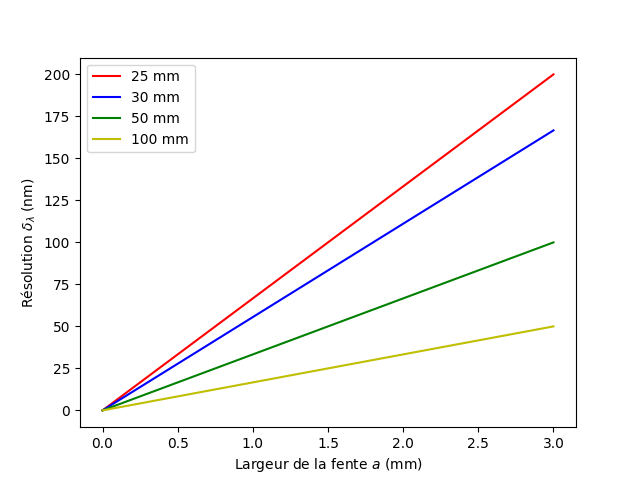
\includegraphics[scale=0.5]{Resolution.png}
    \caption{Résolution du spectromètre en fonction de la largeur de la fente $a$ et de la longueur focale $f_1$}
    \label{res}
\end{figure}
 La figure \ref{arc-en-ciel} montre la simulation de l'équation pour U2 pour les parametres suivants: 
 f1=50mm, f2=25mm, largeur de la fente=0.1mm, longueur de la fente=20mm. Ce résultats est obtenu pour
 60 longueurs d'onde différentes variant du rouge(780nm) au bleu (380nm). 
 \begin{figure}[H]
    \centering
    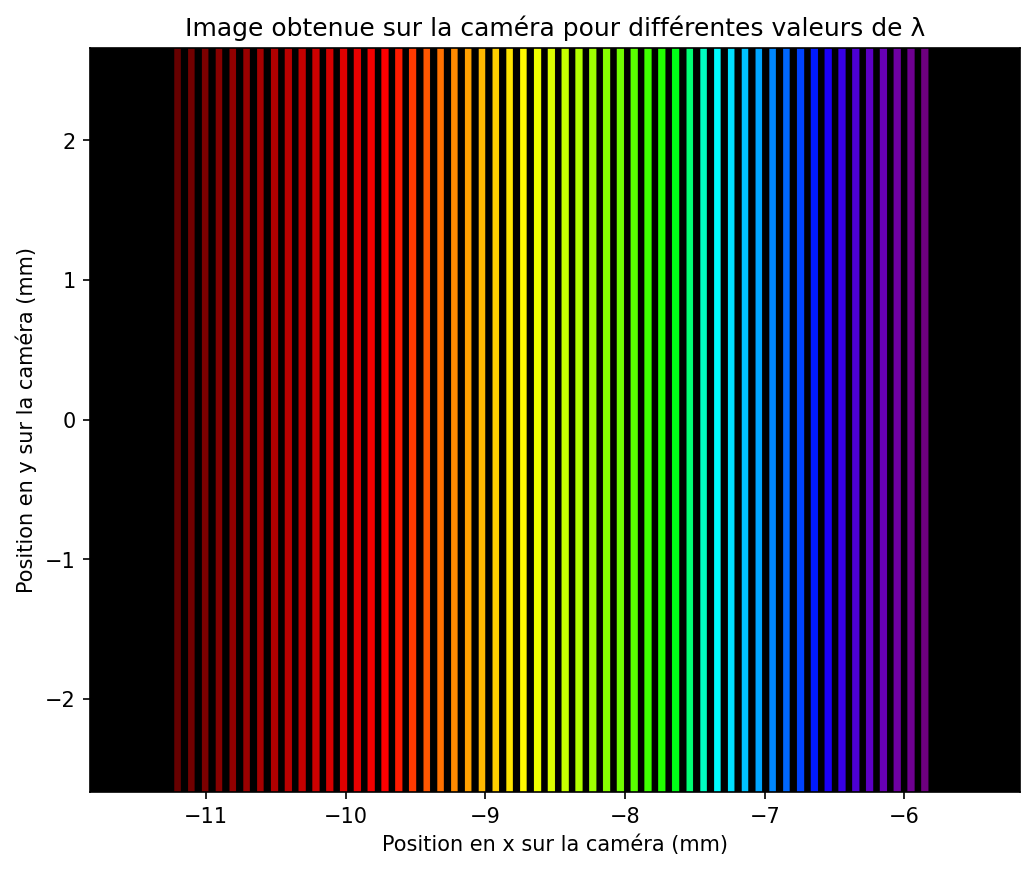
\includegraphics[scale=0.45]{simulation.png}
    \caption{Image appraissant sur la caméra}
    \label{arc-en-ciel}
\end{figure}


L'angle d'incidence sur le réseau de diffraction obtenu avec l'équation \ref{GratingEq}
est $60,3{^\circ}$. Les rayons rouge et bleus diffractés ont un angle de sortie du réseau
de diffraction de $74,4{^\circ}$ et $46,3{^\circ}$ respectivement. La largeur du faisceau
de sortie est de 12,5 mm à une distance de 25,0 mm du réseau de diffraction et la lentille L2
positionnée à cette distance a un diamètre de 12,7 mm. La longueur d'onde centrale est 
$\lambda_c=\frac{\lambda_{bleu}+\lambda_{red}}{2}=580$. À cette longueur d'onde, l'angle de 
diffraction est de $57,5{^\circ}$, ce qui correspond à un angle de $87,2{^\circ}$ entre les deux  

La longueur d'onde diffractée sur l'axe optique est de 621 nm.

\section{Discussion}
Tel que démontré mathématiquement dans la section \ref{methodes}, l'ordre $n=1$ est optimal pour visualiser la diffraction
du faisceau entrant. Physiquement, l'ordre $n=0$ n'est pas pertinent pour le contexte d'un spectromètre parce qu'il ne présente que 
la réflection du faisceau. La diffraction est seulement visible pour les ordres $|n|\geq0$, et ce, avec beaucoup plus d'intensité pour l'ordre $n=1$.
Par conséquent, l'axe optique à la sortie du réseau de diffraction doit être aligné avec l'ordre $n=1$ et non l'ordre $n=0$, ce qui impose
de positionner le réseau de diffraction à un angle particulier. \textcolor{red}{explication de l'angle d'incidence et de sortie}.

En évaluant les résultats des longueurs focales $f_2$ et en considérant la condition initiale
$x(\lambda_{bleu})-x(\lambda_{rouge})\leq 6.656$ mm, les seules lentilles acceptables sont celles
ayant une longueur focale inférieure ou égale à 25 mm. En raison des dimensions physiques des composantes et de
la position du capteur de la caméra, les lentilles ayant des longueurs focales inférieures à 25 mm ne peuvent pas être utilisées.
Ceci élimine donc toutes les lentilles sauf celle de longueur focale $f_2=25$ mm, limitant ainsi le choix à celle-ci.

Pour ce qui est du choix de la longueur focale de la première lentille $f_1$, la relation inversement proportionnelle
entre la résolution et $f_1$ ($\Lambda a/f_1$) permet de déterminer qu'une longueur focale plus grande serait optimale. Cependant,
les limites imposées par l'impression 3D élimine le choix de $f_1=100$ mm. La deuxième longueur focale la plus grande, soit $f_1=50$ mm,
est donc choisie.

La simulation de la modélisation mathématique donne un résultat satisfaisant. En effet, on remarque que tout le spectre
de la lumière visible est présent sur la caméra. Il est cependant important de mentionner qu'il a fallu ajuster la
position de la caméra. Cette manipulation était nécessaire car le modèle mathématique considère que c'est l'ordre 0 qui est placé à 90 degrés du rayon
incident et il faut que ce soit l'ordre 1 qui corresponde à cet alignement. En effet, c'est à l'ordre 1 qu'on peut observer
la diffraction avec la plus forte intensité lumineuse. On remarque également qu'avec les paramètres utilisés, le spectre est plus étroit
que le capteur. Cette situation n'est pas problématique car il est préférable d'avoir le spectre complet plutôt que d'avoir la totalité du capteur utilisée
avec une partie du spectre manquante.

Lors de la simulation, il a été remarqué que c'est le paramètre de la largeur de la fente d'entrée qui a le plus d'impact sur l'image,
car elle a une incidence directe sur la largeur du rectangle de l'image. C'est-à-dire que plus la fente est large, plus
l'image rectangulaire (fente de sortie) sera elle aussi de plus en plus large. La hauteur de la fente n'a quant à elle pas eu d'impact
visible sur l'image. Les longueurs focales sont restées constantes car il s'agit déjà du choix le plus optimal possible.

On peut donc dire que c'est la taille de l'image, soit la largeur de la fente de sortie, qui a le plus d'impact sur la résolution comparée, par exemple, au nombre de pixels
car même pour la largeur de fente d'entrée la plus petite (0.1 mm), la largeur de la fente de sortie reste beaucoup plus large que la largeur du pixel.
Ainsi, dans ce cas, la limitation de la résolution vient de la fente de sortie car si deux longueurs d'onde sont trop proches, les images se superposeront
et rendront ainsi la distinction entre les deux difficile.

Puisque le système utilise des lentilles convergentes, l'impact de l'aberration sphérique \cite{edmund_optics_aberrations} sur la résolution est à considérer.
En effet, lorsqu'un rayon lumineux passe par une lentille convergente, les rayons passant sur les extrémités de la lentille
n'auront pas la même image que les rayons passant par le centre de la lentille. Donc, dans notre cas, ce sont les
rayons dans le rouge ou dans le bleu qui subiront le plus cette abération. Celle-ci a pour effet de légèrement courber l'image
ainsi que de créer un flou dans la périphérie de celle-ci, ce qui affecte par conséquent la résolution du système, surtout pour les longueurs d'onde
extrêmes. 

Cette aberration n'est pas la seule qui affecte différement les longueurs d'onde à imager. En effet, le chromatisme des lentilles
est également une source d'aberrations dans ce montage. Au niveau de la première lentille, ce phénomène 





\clearpage
\printbibliography

\section{Annexes}

\subsection{Développement mathématique détaillé}
yap yap


\clearpage


\end{document}
